\documentclass[UTF8,zihao=-4]{ctexart}
\usepackage{graphicx}
\usepackage{geometry}
\usepackage{siunitx}
\usepackage{amsmath}
\usepackage{amsfonts}
\usepackage{amssymb}
\usepackage{listings}
\lstset{
	language=C++,
	breaklines,
	tabsize=4,
	basicstyle=\ttfamily \small
}
\geometry{a4paper,centering,scale=0.8}
\setCJKfamilyfont{namekai}{AR PL UKai CN}
\title{\heiti 人工智能\quad 第一次作业}
\author{\CJKfamily{namekai} PB17000005\quad 赵作竑}
\date{\kaishu \today}
\begin{document}
	\maketitle
	\begin{itemize}
		\item[3.6]
		\begin{itemize}
			\item[a]
			\textbf{初始状态:}使用图$G$来描述地图,地图上每块对应图$G$上的顶点$G.V[i]$;相邻的两块在图上对应的两个顶点间由边相连。每块的颜色由顶点的颜色属性$V[i].\text{color}$表示。状态为图上的着色状况,也就是图本身。开始时,所有顶点的颜色为none;

			\textbf{可能行动:}Agent将其中一个顶点着色为四种颜色之一;
			
			\textbf{转移模型:}$\text{Paint}(V[i],\text{ColorID})$函数将图中一个顶点$V[i]$着色为ColorID所代表的颜色,返回整个图;

			\textbf{目标测试:}遍历整个图,判断任一顶点是否已全部着色,且与其相邻的顶点的颜色是否相同,若均着色且均不相同,则达到目标;
			\item[b]
			\textbf{初始状态:}两个箱子的位置与高度,猴子的位置与高度,定义了一个状态:
			
			$S(\text{Monkey},\text{Box}_1,\text{Box}_2)$;任一合理状态可能作为一个初始状态。

			\textbf{可能行动:}Monkey移动到某位置,记为$\text{MoveTo(x)}$;Monkey拿起其所处位置的箱子,记为Take;Monkey将其拿的箱子放在其所处的位置,记为PutDown;Monkey攀爬上其所处位置的箱子,记为Up;Monkey攀爬下其所处位置的箱子,记为Down。
			
			\textbf{转移模型:}一组状态经过Monkey的一个动作后变为另一组状态:$S_2=S_1.\text{Action}$,其中Action指Monkey的可能行动。

			\textbf{目标测试:}判断$\text{Monkey}.\text{y} \geq 5$,如果成立,则达到目标。

			\textbf{路径耗散:}Monkey的每个动作有消耗。
			\item[d]
			\textbf{初始状态:}三个水壶中水的容量分别记为$P_1,P_2,P_3$,一个状态定义为一组$P$的取值。初始状态中,$P_1=P_2=P_3=0$。

			\textbf{可能行动:}将一个水壶倒满水;将一个水壶中的水倒到另一个水壶中,直到水壶中的水倒光或者另一个水壶倒满;将一个水壶的水全部倒到地上。
			
			\textbf{转移模型:}一组状态经过一个行动变为另一组状态。返回该状态。

			\textbf{目标测试:}遍历三个水壶,若某一水壶中水的体积是1加仑,则达到目标。

			\textbf{路径耗散:}每次倒水的消耗为1。
		\end{itemize} 
		\item[3.9]
		\begin{itemize}
			\item[a]
			\textbf{状态:}左河岸上传教士和野人的人数,以及船的位置,构成了状态;
			
			\textbf{初始状态:}左河岸上传教士和野人的人数都是3,船在左河岸;

			\textbf{可能行动:}将$m$个传教士和$n$个野人从船所在的河岸运送到河的对岸,记左岸的传教士为$x$个,野人为$y$个。一次运送满足$2\geq m+n\geq 1$;若船在左岸,则$x-m=0$或$x-m\geq y-n$,且$3-x+m=0$或$3-x+m\geq 3-y+n$;
			
			\textbf{转移模型:}由一个状态经过一次转换到达另一个状态;

			\textbf{目标测试:}到达的状态为目标状态($x=0,y=0,b=r$);

			\textbf{路径耗散:}每次的行动的消耗为1。

			完整的状态空间图见图\ref{all}。三个参数$(x,y,b)$分别表示左岸传教士和野人的个数,以及船的位置。

			\begin{table}
				\centering
				\begin{tabular}{cccc}
					$(0,0,l)$ & $(1,0,l)$ & $(2,0,l)$ & $(3,0,l)$ \\
					$(0,0,r)$ & $(1,0,r)$ & $(2,0,r)$ & $(3,0,r)$ \\
					$(0,1,l)$ & $(1,1,l)$ & $(2,1,l)$ & $(3,1,l)$ \\
					$(0,1,r)$ & $(1,1,r)$ & $(2,1,r)$ & $(3,1,r)$ \\
					$(0,2,l)$ & $(1,2,l)$ & $(2,2,l)$ & $(3,2,l)$ \\
					$(0,2,r)$ & $(1,2,r)$ & $(2,2,r)$ & $(3,2,r)$ \\
					$(0,3,l)$ & $(1,3,l)$ & $(2,3,l)$ & $(3,3,l)$ \\
					$(0,3,r)$ & $(1,3,r)$ & $(2,3,r)$ & $(3,3,r)$ \\
				\end{tabular}
				\caption{完整的状态空间图}
				\label{all}
			\end{table}

			\item[b] 使用广度优先搜索解决问题,编写代码并运行程序,可以得到结果11。

			虽然对于广度优先搜索算法而言,出现循环并不影响求出最优解,所以不是必须的,但是通过避免重复状态可以减少搜索的时间。

			最优解可见图\ref{moving}。
			\begin{lstlisting}
/*
* Solve the problem about Missionaries and Cannibals with BFS
* This file is created by Zhao Zuohong on Feb 25, 2020
* All rights reserved.
*/

#include <cstdio>
#include <cstring>

// two directions
const int l = 0;
const int r = 1;

// if a status is considered
int Marked[4][4][2];

// the status
typedef struct status {
	int x; // num of missionaries
	int y; // num of cannibals
	int b; // location of boat
	int moves; // to hold the result
} status;

// begin and target
status begin = { 3, 3, l, 0 };
status target = { 0, 0, r, 0 };

// Queue of status
const int QLimit = 100;
status Queue[QLimit];
int QLength;
int QHead;

void EnQueue(status s)
{
	Queue[(QHead + QLength) % QLimit] = s;
	QLength = (QLength + 1) % QLimit;
}

bool DeQueue(status* s)
{
	if (QLength == 0) {
		return false;
	}
	*s = Queue[QHead];
	QHead = (QHead + 1) % QLimit;
	--QLength;
	return true;
}

void init(void)
{
	EnQueue(begin);
}

// check whether a move of m missionaries and n cannibals is valid
bool CheckMove(status* s, int m, int n)
{
	int leftx, lefty, rightx, righty;
	if (s->b == l) {
		leftx = s->x - m;
		lefty = s->y - n;
		rightx = 3 - s->x + m;
		righty = 3 - s->y + n;
	} else {
		leftx = s->x + m;
		lefty = s->y + n;
		rightx = 3 - s->x - m;
		righty = 3 - s->y - n;
	}
	if (leftx != 0) {
		if (leftx < lefty) {
			return false;
		}
	}
	if (rightx != 0) {
		if (rightx < righty) {
			return false;
		}
	}
	return true;
}

// check whether the agent has reached the target
bool ReachTarget(status s)
{
	if (s.x == target.x && s.y == target.y && s.b == target.b) {
		return true;
	} else {
		return false;
	}
}

// bfs algorithm to solve this problem
int bfs(void)
{
	status current_status;
	while (DeQueue(&current_status)) {
		int mlimit, nlimit; // range of m and n
		if (current_status.b == l) {
			mlimit = current_status.x;
			nlimit = current_status.y;
		} else {
			mlimit = 3 - current_status.x;
			nlimit = 3 - current_status.y;
		}
		for (int m = 0; m <= mlimit; ++m) {
			for (int n = 0; n <= nlimit; ++n) {
				if (m == 0 && n == 0) {
					continue;
				}
				if (m + n > 2) {
					continue;
				}
				if (CheckMove(&current_status, m, n)) {
					status new_status; // transfer from current state to new state
					if (current_status.b == l) {
						new_status.b = r;
						new_status.x = current_status.x - m;
						new_status.y = current_status.y - n;
					} else {
						new_status.b = l;
						new_status.x = current_status.x + m;
						new_status.y = current_status.y + n;
					}

					if (Marked[new_status.x][new_status.y][new_status.b] == 1) {
						continue;
					}
					Marked[new_status.x][new_status.y][new_status.b] = 1;

					new_status.moves = current_status.moves + 1;
					if (ReachTarget(new_status)) {
						return new_status.moves;
					}
					EnQueue(new_status);
				}
			}
		}
	}
	return -1;
}

int main(void)
{
	init();
	int result = bfs();
	printf("%d\n", result);
	return 0;
}
			\end{lstlisting}
			\begin{figure}[htbp]
				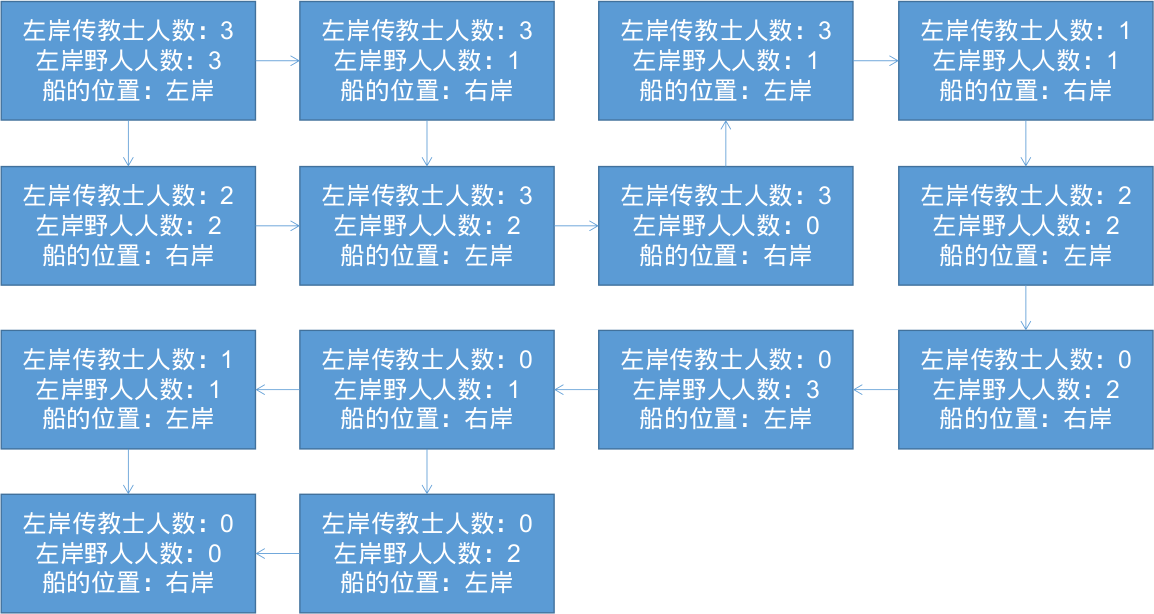
\includegraphics[width=\textwidth]{Moving.png}
				\label{moving}
			\end{figure}
			\item[c] 可能有几个原因:一是正确理解题意,二是推导步数比较多,三是约束较多,判断条件比较复杂。
		\end{itemize}  
	\end{itemize}
\end{document}